\documentclass{standalone}
\usepackage{amsmath}
\usepackage{tikz}
\begin{document}
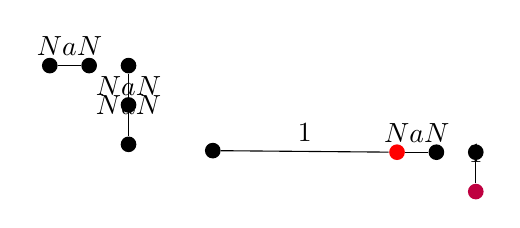
\begin{tikzpicture}
\node[fill=black, circle, inner sep=2pt, label=above:{\textcolor{black}{$$}}] (G1N0) at (5.77,-1.28) {};
\node[fill=red, circle, inner sep=2pt, label=above:{\textcolor{red}{$$}}] (G1N1) at (8.11,-1.3) {};
\node[fill=black, circle, inner sep=2pt, label=above:{\textcolor{black}{$$}}] (G1Nsigma male) at (8.61,-1.3) {};
\node[fill=black, circle, inner sep=2pt, label=above:{\textcolor{black}{$$}}] (G1N2) at (9.11,-1.3) {};
\node[fill=purple, circle, inner sep=2pt, label=above:{\textcolor{purple}{$$}}] (G1N3) at (9.11,-1.8) {};
\draw[draw=black, shorten >=0pt, shorten <=0pt] (G1N0) -- (G1N1) node[midway, above] {\textcolor{black}{$1$}};
\draw[draw=black, shorten >=0pt, shorten <=0pt] (G1N1) -- (G1Nsigma male) node[midway, above] {\textcolor{black}{$NaN$}};
\draw[draw=black, shorten >=0pt, shorten <=0pt] (G1N2) -- (G1N3) node[midway, above] {\textcolor{black}{$1$}};
\node[fill=black, circle, inner sep=2pt, label=above:{\textcolor{black}{$$}}] (G2NA) at (3.7,-0.2) {};
\node[fill=black, circle, inner sep=2pt, label=above:{\textcolor{black}{$$}}] (G2Nbeta) at (4.2,-0.2) {};
\node[fill=black, circle, inner sep=2pt, label=above:{\textcolor{black}{$$}}] (G2ND) at (4.7,-0.2) {};
\node[fill=black, circle, inner sep=2pt, label=above:{\textcolor{black}{$$}}] (G2NB) at (4.7,-0.7) {};
\node[fill=black, circle, inner sep=2pt, label=above:{\textcolor{black}{$$}}] (G2NC) at (4.7,-1.2) {};
\draw[draw=black, shorten >=0pt, shorten <=0pt] (G2NA) -- (G2Nbeta) node[midway, above] {\textcolor{black}{$NaN$}};
\draw[draw=black, shorten >=0pt, shorten <=0pt] (G2NB) -- (G2NC) node[midway, above] {\textcolor{black}{$NaN$}};
\draw[draw=black, shorten >=0pt, shorten <=0pt] (G2NC) -- (G2ND) node[midway, above] {\textcolor{black}{$NaN$}};
\end{tikzpicture}
\end{document}
